\section{Teorema de Stokes. Teorema de la divergencia de Gauss}


\subsection{Teorema de Stokes}

\begin{definición} [Rotacional]
    Sean $A \subset \mathbb{R}^3$ un conjunto abierto y $\vec{F} : A \to \mathbb{R}^3$ un campo vectorial de clase $C^1$. Se define el rotacional de $\vec{F} = (F_1,F_2,F_3)$ como:
    $$ rot(\vec{F}) = \nabla \times \vec{F} = \begin{vmatrix}
        \vec{e}_1 & \vec{e}_2 & \vec{e}_3 \\
        \frac{\partial}{\partial x} & \frac{\partial}{\partial y} & \frac{\partial}{\partial z} \\
        F_1 & F_2 & F_3
        \end{vmatrix} = \left( \frac{\partial F_3}{\partial y} - \frac{\partial F_2}{\partial z}, \frac{\partial F_1}{\partial z} - \frac{\partial F_3}{\partial x}, \frac{\partial F_2}{\partial x} - \frac{\partial F_1}{\partial y} \right)
    $$
\end{definición}

\begin{observación}
    En este caso, $rot(\vec{F})$ es un campo vectorial continuo definido en $A$.
\end{observación}

\ejemplo{
    Sea $(P,Q) : U \to \mathbb{R}^2$ un campo vectorial de clase $C^1$ definido en un abierto $U \subset \mathbb{R}^2$. Consideramos $A = U \times \mathbb{R}$ y el campo vectorial $\vec{F} = (P,Q,0)$. Entonces el rotacional de $\vec{F}$ es:
    $$ \nabla \times \vec{F} = \begin{vmatrix}
        \vec{e}_1 & \vec{e}_2 & \vec{e}_3 \\
        \frac{\partial}{\partial x} & \frac{\partial}{\partial y} & \frac{\partial}{\partial z} \\
        P & Q & 0
    \end{vmatrix} = \left( 0, 0, \frac{\partial Q}{\partial x} - \frac{\partial P}{\partial y} \right) \qquad \text{"la derivación del toerema de Green"}$$
}

\begin{teorema} [Teorema de Stokes]
    Sea $(S, \vec{n})$ una superficie orientada y regular a trozos, y sea $\vec{F}$ un campo vectorial de clase $C^1$ definido en un abierto $U \supset S$. Entonces se cumple la siguiente igualdad:
    $$ \int_{(S, \vec{n})} rot(\vec{F}) = \int_{\partial S} \vec{F} $$
    donde $\partial S$ tiene la orientación inducida por $\vec{n}$.
\end{teorema}

\ejemplo{
    Sea la superficie $S = \{(x,y,z) \in \mathbb{R}^3 : z = x^2 + y^2 \leq 4\}$ con la norma exterior $\vec{n}$ y el campo vectorial $\vec{F} = (yz, -xz, z)$. Verificamos el teorema de Stokes.\\
    Tenemos que $\partial S = \{(x,y,z) \in \mathbb{R}^3 : z = x^2 + y^2 = 4\}$, que es una circunferencia de radio $2$ en el plano $z=4$. Fijémonos que $\vec{n}$ induce la orientación negativa en la curva $C^- = \partial S$.
    \begin{center}
        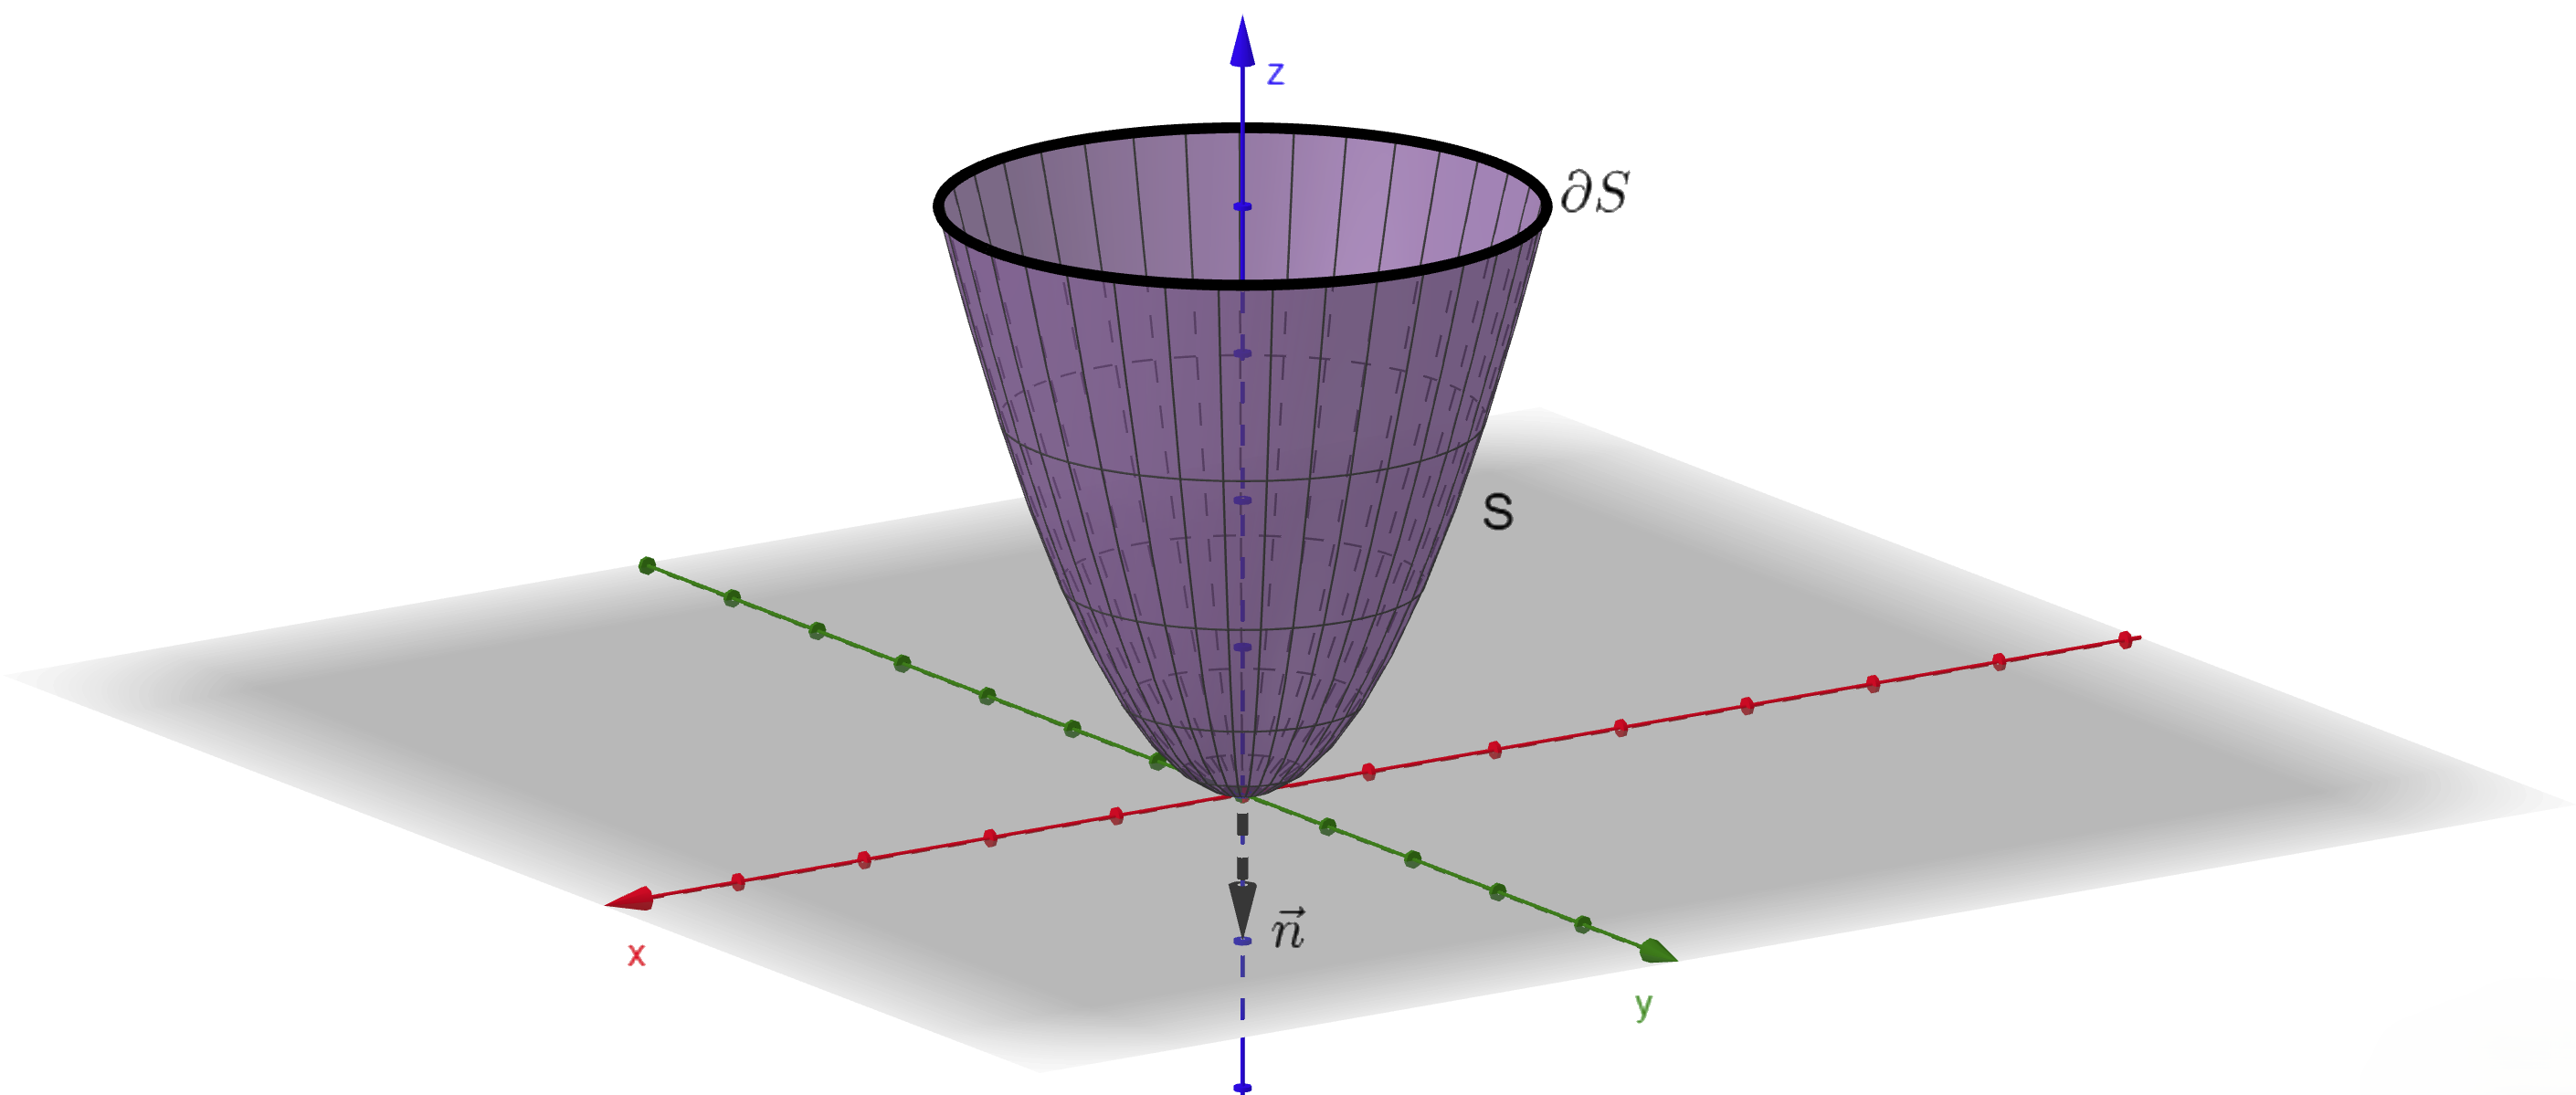
\includegraphics[width=0.65\linewidth]{images/ej4.png}
    \end{center}   
    El rotacional de $\vec{F}$ es:
    $$ rot(\vec{F}) = \nabla \times \vec{F} = \begin{vmatrix}
        \vec{e}_1 & \vec{e}_2 & \vec{e}_3 \\
        \frac{\partial}{\partial x} & \frac{\partial}{\partial y} & \frac{\partial}{\partial z} \\
        yz & -xz & z
    \end{vmatrix} = \left( x, y, -2z \right)$$
    Consideramos la parametrización natural $\varphi : D \to S$ de $S$ dada por:
    $$ \varphi(x,y) = \begin{cases}
        x = x \\
        y = y \\
        z = x^2 + y^2
    \end{cases} \qquad \text{donde } D = \{(x,y) \in \mathbb{R}^2 : x^2 + y^2 \leq 4\}$$
    Entonces la normal a la superficie $S$ es:
    $$ \vec{N}_\varphi =
        \begin{vmatrix}
            \vec{e}_1 & \vec{e}_2 & \vec{e}_3 \\
            1         & 0         & 2x        \\
            0         & 1         & 2y
        \end{vmatrix} = (-2x, -2y, 1)$$
    La normal $\vec{N}_\varphi$ apunta hacia arriba en el punto $(0,0,0)$, luego tenemos una normal interior.
    \begin{itemize}
        \item Calculamos el rotacional de $\vec{F}$ en $S$ por medio de la parametrización $\varphi$:
        $$\int_{(S, \vec{n})} rot(\vec{F}) = -\int_{D} \langle \vec{N}_\varphi, rot(\vec{F}) \circ \varphi(x,y) \rangle dx dy = -\int_{D} \langle (-2x, -2y, 1), (x,y,-2(x^2+y^2) \rangle dx dy$$
        $$ = \int_{D} 2x^2 + 2y^2 + 2x^2 + 2y^2 dx dy = \int_{D} 4(x^2+y^2) dx dy = 4 \int_{\theta=0}^{\theta=2\pi} \int_{r=0}^{r=2} r^2 \cdot r \, dr \, d\theta$$ 
        $$= 4 \cdot 2\pi \left[ \frac{r^4}{4} \right]_{r=0}^{r=2} = 4 \cdot 2\pi \cdot 4 = 32\pi$$
        \item Consideramos la parametrización positiva $\gamma$ de la curva $\partial S$ dada por:
        $$ \gamma(t) = \begin{cases}
            x = 2 \cos(t) \\
            y = 2 \sin(t) \\
            z = 4
        \end{cases} \qquad \text{donde } t \in [0,2\pi]$$
        y calculamos la integral de línea del campo $\vec{F}$ sobre la curva $\partial S$:
        $$\int_{\partial S} \vec{F} = \int_{C^-} \vec{F} = -\int_{\gamma} \vec{F} = -\int_{t=0}^{t=2\pi} \langle \vec{F}(\gamma(t)), \gamma'(t) \rangle dt $$
        $$= -\int_{t=0}^{t=2\pi} \langle (8 \sin(t), -8 \cos(t), 4), (-2 \sin(t), 2 \cos(t), 0) \rangle dt$$
        $$= \int_{t=0}^{t=2\pi} 16 dt = 16 \left[ t \right]_{t=0}^{t=2\pi} = 16(2\pi - 0) = 32\pi$$
    \end{itemize}
    En efecto, vemos que las integrales coinciden de acorde al teorema de Stokes.
}

\ejemplo{
    Sea $S = S_1 \cup S_2$, donde:
    $$
        S_1 = \{(x,y,z) \in \mathbb{R}^3 : x^2 + y^2 = 1, \ z \in [0,2] \}
        \qquad
        S_2 = \{(x,y,z) \in \mathbb{R}^3 : z = 2, \ x^2 + y^2 \leq 1 \}
    $$
    con la norma exterior $\vec{n}$ y el campo vectorial $\vec{F}(x,y,z) = (y,x,z)$. 
    El borde de $S$ es:
    $$ \partial S = C_0^+ = \{(x,y,z) \in \mathbb{R}^3 : x^2 + y^2 = 1, \ z = 0 \}$$
    \begin{center}
        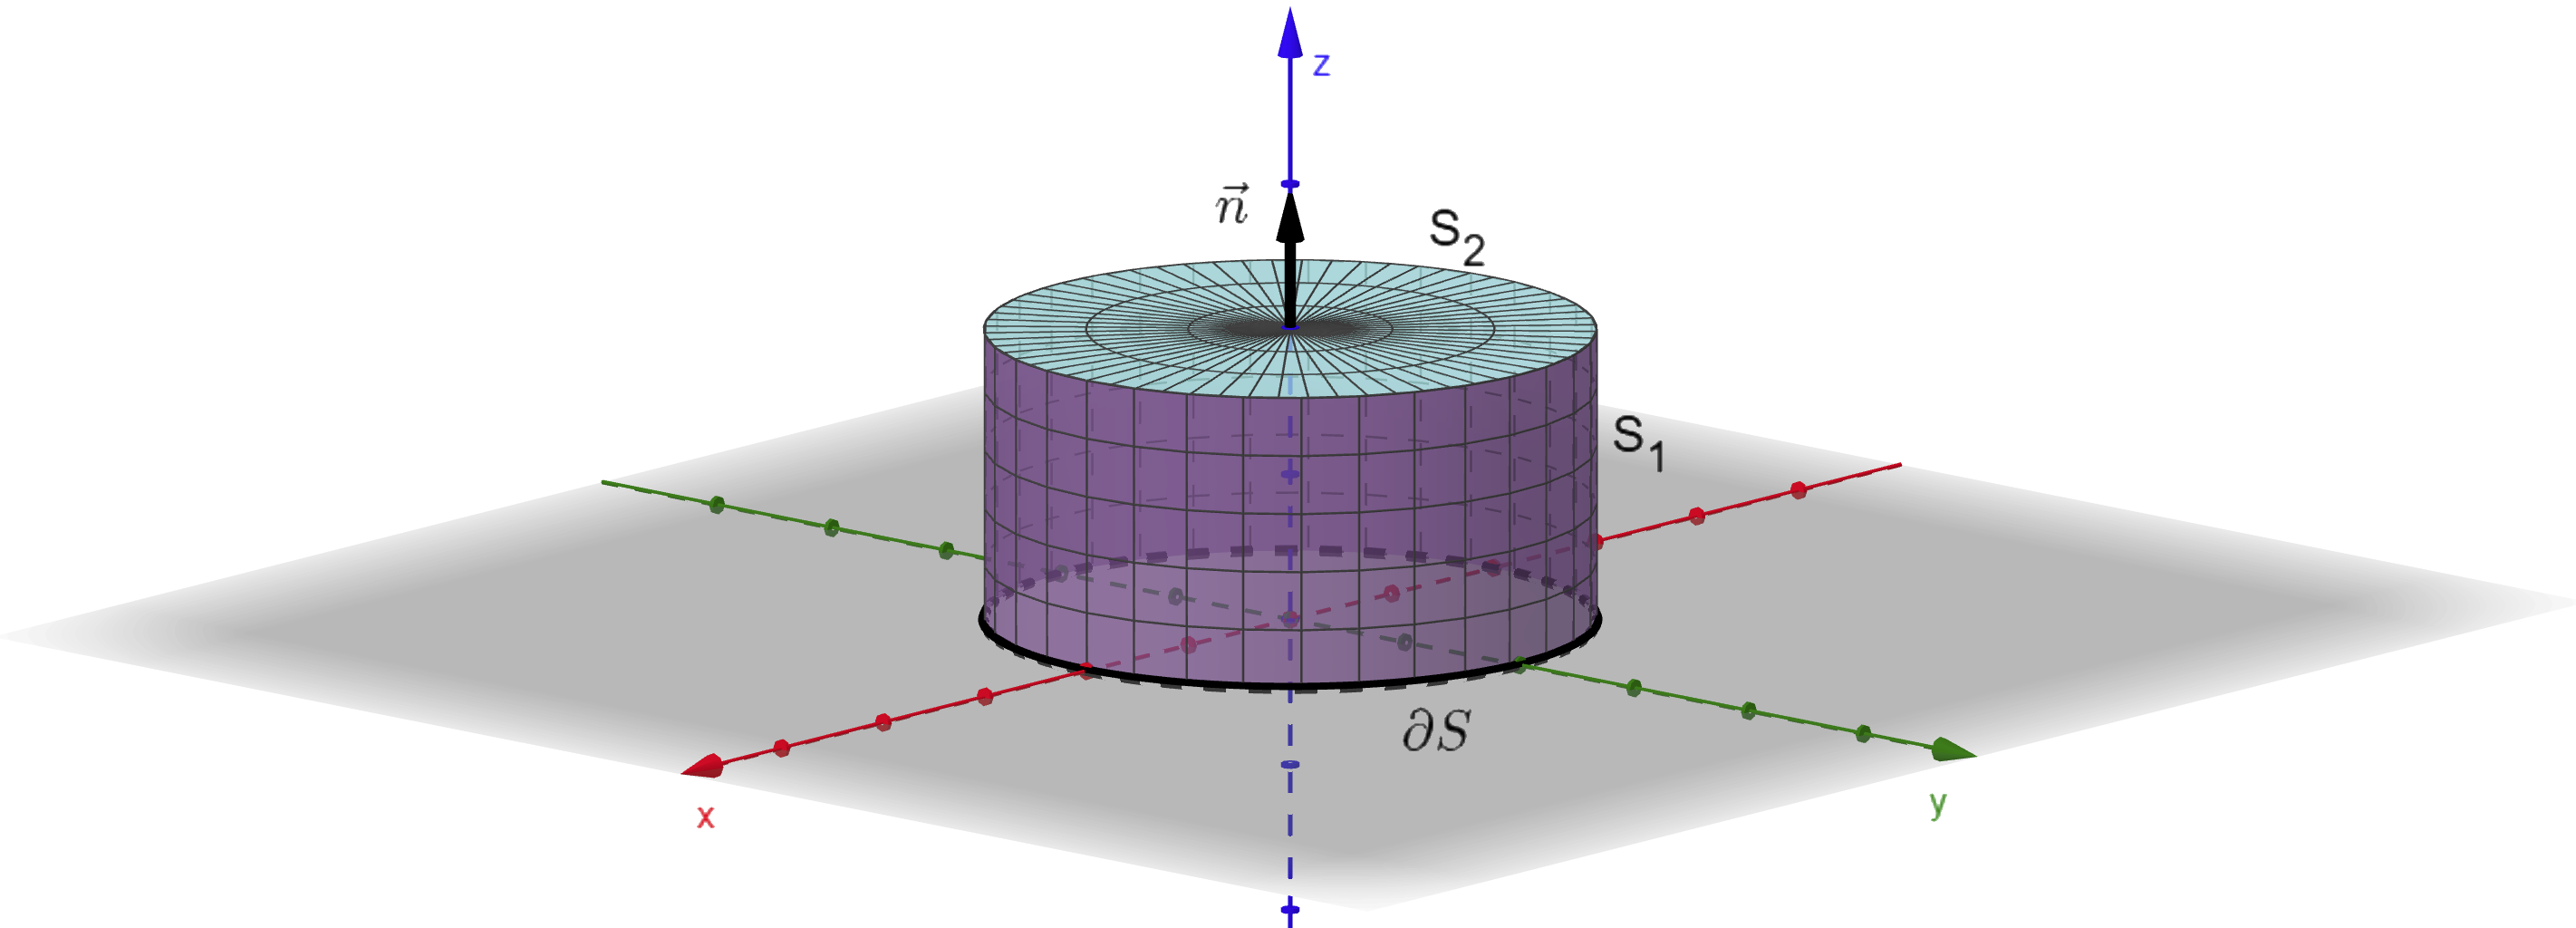
\includegraphics[width=0.65\linewidth]{images/ej5.png}
    \end{center} 
    Calculamos el rotacional del campo $\vec{F}$:
    $$ rot(\vec{F}) = \nabla \times \vec{F} = \begin{vmatrix}
        \vec{e}_1 & \vec{e}_2 & \vec{e}_3 \\
        \frac{\partial}{\partial x} & \frac{\partial}{\partial y} & \frac{\partial}{\partial z} \\
        y & x & z
    \end{vmatrix} = \left( 0, 0, 1 - 1 \right) = (0,0,0)$$
    Consideramos la parametrización $\gamma$ de la curva $C_0$ dada por:
    $$ \gamma(t) = \begin{cases}
        x = \cos(t) \\
        y = \sin(t) \\
        z = 0
    \end{cases} \qquad \text{donde } t \in [0,2\pi]$$
    que tiene orientacion positiva. Además, $\gamma'(t) = (-\sin(t), \cos(t), 0)$.
    \begin{itemize}
        \item Calculamos la integral del campo $rot(\vec{F})$ sobre la superficie $S$:
        $$\int_{(S, \vec{n})} rot(\vec{F}) = \int_{(S_1, \vec{n}_1)} \vec{0} = 0$$
        \item Hacemos la integral de línea del campo $\vec{F}$ sobre la curva $C_0^+$:
        $$\int_{\partial S} \vec{F} = \int_{C_0^+} \vec{F} = \int_{t=0}^{t=2\pi} \langle (\sin(t), \cos(t), 0), (-\sin(t), \cos(t), 0) \rangle dt$$
        $$= \int_{t=0}^{t=2\pi} \cos^2(t) - \sin^2(t) dt = \int_{t=0}^{t=2\pi} \cos(2t) dt = \left[ \frac{\sin(2t)}{2} \right]_{t=0}^{t=2\pi} = 0$$
    \end{itemize}
    Vemos que el teorema de Stokes se cumple, ya que las integrales son iguales.
}

\ejemplo{
    Consideramos el campo vectorial $\vec{F} = (yz, -xz, z)$. Veamos el rotacional de $\vec{F}$:
    $$ rot(\vec{F}) = \nabla \times \vec{F} = \begin{vmatrix}
        \vec{e}_1 & \vec{e}_2 & \vec{e}_3 \\
        \frac{\partial}{\partial x} & \frac{\partial}{\partial y} & \frac{\partial}{\partial z} \\
        yz & -xz & z
    \end{vmatrix} = \left( x, y, -2z \right)$$
    Supongamos que tenemos una superficie $S$ cualesquiera cuyo borde $\partial S$ sea la curva $C_0^+$ del ejemplo anterior. Entonces tenemos que:
    $$ \int_{(S, \vec{n})} rot(\vec{F}) = \int_{C_0^+} \vec{F} = \int_{C_0^+} \vec{F} = \int_{t=0}^{t=2\pi} \langle (0,0,0), (-\sin(t), \cos(t), 0) \rangle dt = 0$$
}

\begin{observación}
    Si $S$ es una superficie cerrada, es decir, $\partial S = \emptyset$, entonces se tiene que:
    $$ \int_{(S, \vec{n})} rot(\vec{F}) = \int_{\partial S} \vec{F} = 0$$
\end{observación}

\subsection{Geometria del Rotacional}

\ejemplo{
    Sea $\vec{F: U \to \mathbb{R}^2}$ el campo de velocidades de un fluido en $\mathbb{R}^2$. Las trayectorias son curvas $\gamma: I \to U$ con $\gamma'(t) = \vec{F}(\gamma(t))$.
}

\ejemplo{
    Sean $U \subset \mathbb{R}^3$ abierto y $\vec{F} : U \to \mathbb{R}^3$ un campo vectorial de clase $C^1$.\\
    Consideremos $p \in U$ y $r > 0$, siendo $D_r$ el circulo de centro $p$ y radio $r$, con frontera $C_r = \partial D_r$.\\
    Sea $\vec{u}$ un vector unitario de $\mathbb{R}^3$ perpendicular al plano que contiene a $D_r$, entonces:
    $$ \langle rot(\vec{F}) (p), \vec{u} \rangle = \lim_{r \to 0} \frac{1}{\pi r^2} \int_{C_r^+} \vec{F} $$
    Donde $C_r^+$ denota a $C_r$ conla orientacion comparativa a la de $\vec{u}$, y donde esta igualdad representa la "circulacion por unidad de área" del campo $\vec{F}$.   
}

\begin{proof}
    $$ \int_{C_r^+} \vec{F} = \int_{(D_r, \vec{n})} rot\vec{F} = \int_{D_r} \langle \vec{F}, \vec{u} \rangle = \int_{D_r} \langle rot\vec{F} - rot\vec{F} (p), \vec{u} \rangle + \langle rot\vec{F} (p), \vec{u} \rangle$$
    De donde pasamos a:
    $$ \int_{D_r} \langle rot\vec{F} (p), \vec{u} \rangle_{\text{constante}} = \langle rot\vec{F} (p), \vec{u} \rangle \cdot \text{área}(D_r)$$
    Entonces:
    $$ \forall \epsilon > 0, \quad \exists \delta > 0: \quad 0 < r < \delta \implies \lVert rot\vec{F} (x,y,z) - rot\vec{F} (p) \rVert < \epsilon \quad \forall (x,y,z) \in D_r \implies $$
    $$ \implies \left| \int_{D_r} \langle rot\vec{F} - rot\vec{F} (p), \vec{u} \rangle \right| \leq \int_{D_r} \left| \langle rot\vec{F} - rot\vec{F} (p), \vec{u} \rangle \right| \leq \int_{D_r} \lVert rot\vec{F} - rot\vec{F} (p) \rVert \leq \epsilon \cdot \text{área}(D_r)$$
    Luego:
    $$ \left| \frac{1}{\text{área}(D_r)} \int_{C_r^+} \vec{F} - \langle rot\vec{F} (p), \vec{u} \rangle \right| < \epsilon \quad \forall 0 < r < \delta$$
\end{proof}

\begin{definición}
    Sean $A \subset \mathbb{R}^3$ un conjunto abierto y $\vec{F} : A \to \mathbb{R}^3$ un campo vectorial de clase $C^1$. Se dice que $\vec{F}$ es irrotacional en $A$ si $rot(\vec{F}) \equiv 0$ en $A$.
\end{definición}

\begin{lema}
    Si $\vec{F}$ es un campo de clase $C^1$, y es conservativo en $A$ $\implies$ es irrotacional en $A$.
\end{lema}

\begin{proof}
    Sea $\varphi: A \to \mathbb{R}$ una función tal que $\vec{F} = \nabla \varphi$, es decir, $\vec{F} = \left( \frac{\partial \varphi}{\partial x}, \frac{\partial \varphi}{\partial y}, \frac{\partial \varphi}{\partial z} \right)$, entonces $\varphi$ es de clase $C^2$ en $A$ y, aplicando el teorema de Schwarz, tenemos que:
    $$ rot(\vec{F}) = \nabla \times \nabla \varphi = \begin{vmatrix}
        \vec{e}_1 & \vec{e}_2 & \vec{e}_3 \\
        \frac{\partial}{\partial x} & \frac{\partial}{\partial y} & \frac{\partial}{\partial z} \\
        \frac{\partial \varphi}{\partial x} & \frac{\partial \varphi}{\partial y} & \frac{\partial \varphi}{\partial z}
    \end{vmatrix} = \left( \frac{\partial^2 \varphi}{\partial y \partial z} - \frac{\partial^2 \varphi}{\partial z \partial y}, \frac{\partial^2 \varphi}{\partial z \partial x} - \frac{\partial^2 \varphi}{\partial x \partial z}, \frac{\partial^2 \varphi}{\partial x \partial y} - \frac{\partial^2 \varphi}{\partial y \partial x} \right) = (0,0,0)$$
\end{proof}

\begin{teorema}
    Sea $U \subset \mathbb{R}^3$ un abierto conexo, y sea $\vec{F} : U \to \mathbb{R}^3$ un campo vectorial de clase $C^1$. Entonces son equivalentes las siguientes afirmaciones:
    \begin{enumerate}
        \item $\vec{F}$ es conservativo en $U$.
        \item $\int_\sigma \vec{F} = 0$, $\forall \sigma$ camino triangular en $U$.
        \item $\vec{F}$ es irrotacional en $U$, es decir, $rot(\vec{F}) \equiv 0$ en $U$.
    \end{enumerate}
\end{teorema}

\begin{proof}
    \leavevmode
    \begin{itemize}
        \item (1) $\implies$ (2): Ya esta probado por la caracterizacion de los campos conservativos.
        \item (2) $\implies$ (1): Fijamos un punto $P \in U$ y consideramos para cada $x \in U$ la función
        $$ \varphi(x) = \int_{[P,x]} \vec{F}$$
        Veamos que $\varphi$ es un potencial de $\vec{F}$. Para ellos, veamos que $F_i = \frac{\partial \varphi}{\partial x_i} \ \forall i = 1,2,3$.
        $$ \lim_{h \to 0} \frac{1}{h} \left(\underbrace{\int_{[P,x + h\vec{e}_i]} \vec{F}}_{\varphi(x+h\vec{e}_i)} - \underbrace{\int_{[P,x]} \vec{F}}_{\varphi(x)} \right) = \lim_{h \to 0} \frac{1}{h} \left( \varphi(x + h\vec{e}_i) - \varphi(x) \right)$$
        Por (2), tenemos que el triangulo T de vértices $P$, $x$ y $x + h\vec{e}_i$ es tal que 
        $$\int_{[P,x] + [x,x + h\vec{e}_i] + [x + h\vec{e}_i,P]} \vec{F} = 0$$
        Luego se sigue entonces que: 
        $$ \int_{[P,x + h\vec{e}_i]} \vec{F} - \int_{[P,x]} \vec{F} = \int_{[x,x + h\vec{e}_i]} \vec{F}$$
        por tanto 
        $$\frac{1}{h} \int_{[x,x + h\vec{e}_i]} \vec{F} = \frac{1}{h} \int_{t =0}^{t=1} \langle \vec{F}(x + t h \vec{e}_i), h \vec{e}_i \rangle dt = \int_{t=0}^{t=1} \vec{F}_i(x + t h \vec{e}_i)dt \xrightarrow{h \to 0} \vec{F}_i(x)$$
        donde $\gamma(t) = x + t h \vec{e}_i$ con $t \in [0,1]$. Así obtenemos que $(1) \iff (2)$.
        \item $(3) \implies (2)$: Sea $T \subset U$ un triángulo, y sea $ \sigma = \partial T$:
        \item[] $$ \int_\sigma \vec{F} = \int_{(T, \vec{n})} rot(\vec{F}) = 0$$
    \end{itemize}
\end{proof}

\ejemplo{
    Es importante que $U$ sea convexo:\\
    Seam $U = \{(x,y,z) \in \mathbb{R}^3 : (x,y) \neq (0,0) \}$ y $\vec{F}: U \to \mathbb{R}^3$ el campo vectorial dado por:
    $$ \vec{F}(x,y,z) = \left( \frac{-y}{x^2 + y^2}, \frac{x}{x^2 + y^2}, 0 \right) = \left(P,Q,0\right)$$
    Asi tenemos el siguiente rotacional
    $$ rot(\vec{F}) = \begin{vmatrix}
        \vec{e}_1 & \vec{e}_2 & \vec{e}_3 \\
        \frac{\partial}{\partial x} & \frac{\partial}{\partial y} & \frac{\partial}{\partial z} \\
        P & Q & 0
    \end{vmatrix} = \left(0, 0, \frac{\partial Q}{\partial x} - \frac{\partial P}{\partial y}\right) = (0,0,0)$$
    El campo $\vec{F}$ es por tanto irrotacional en $U$, pero $\vec{F}$ no es conservativo. Consideremos la curva cerrada $\gamma$ dada por:
    $$ \gamma(t) = (\cos(t), \sin(t), 0), \quad t \in [0,2\pi] \implies \int_\gamma \vec{F} = \int_{t=0}^{t=2\pi} \langle \vec{F}(\gamma(t)), \gamma'(t) \rangle dt $$
    $$ = \int_{t=0}^{t=2\pi} \langle \left( \frac{-\sin(t)}{1}, \frac{\cos(t)}{1}, 0 \right), (-\sin(t), \cos(t), 0) \rangle dt = \int_{t=0}^{t=2\pi} 1 dt = 2\pi \neq 0$$
    Demostrando así que $\vec{F}$ no es conservativo.
}

\ejemplo{
    \underline{El ejercicio de Nash}:\\
    Encontrar $X \subset \mathbb{R}^3$ tal que si denotamos por 
    $$V = \{ \vec{F}: \mathbb{R}^3  \setminus X \to \mathbb{R}^3  \text{ campo } C^1 \mid rot(\vec{F}) = \vec{0} \}$$
    $$W = \{\vec{F}: \mathbb{R}^3  \setminus X \to \mathbb{R}^3  \text{ campo }C^1 \mid \vec{F} = \nabla g \text{ para algún } g \}$$
    obtengamos que $dim(V \setminus W) = 8$.
}